\documentclass{article}
\usepackage{graphicx, amsmath, amssymb, mathtools, fancyhdr} % Required for inserting images

\graphicspath{{Images/}}

\setlength{\oddsidemargin}{0in}
\setlength{\textwidth}{6.5in}
\setlength{\topmargin}{-.55in}
\setlength{\textheight}{9in}
\pagestyle{fancy}

\fancyfoot{}
\fancyhead[R]{\thepage}
\fancyhead[L]{MATH 6440}

\newcommand{\Res}[1]{\underset{z = #1}{\text{Res}}}



\begin{document}

\begin{center}
    {\huge Homework 3}
    \vspace{0.5cm}

    {\large Michael Nameika}
\end{center}

\begin{itemize}
    \item[6.1.3] Find the asymptotic expansions for the following integrals:
    \begin{itemize}
        \item[(a)] ${\displaystyle \int_0^1\frac{\sin(kt)}{t}dt}$, $k \to 0$.
        \newline\newline
        \textit{Soln.} Note that $\frac{\sin(kt)}{t}$ has a removable singularity at $t = 0$ and that 
        \[\sin(kt) = \sum_{n = 0}^{\infty}\frac{(-1)^n(kt)^{2n+1}}{(2n+1)!}\]
        so that 
        \[\frac{\sin(kt)}{t} = k\sum_{n = 0}^{\infty}\frac{(-1)^n(kt)^{2n}}{(2n+1)!}.\]
        Since the above power series has the same coefficients as the power series for $\sin(t)$, we have the above power series converges for all $t \in \mathbb{R}$. Thus, we can interchange the summation and the integral, so that
        \begin{align*}
            \int_0^1 \frac{\sin(kt)}{t}dt &= \int_0^1 k\sum_{n = 0}^{\infty} \frac{(-1)^n(kt)^{2n}}{(2n + 1)!}dt\\
            &= k\sum_{n = 0}^{\infty}\frac{(-1)^n}{(2n + 1)!}\int_0^1(kt)^{2n}dt\\
            &= k\sum_{n = 0}^{\infty}\frac{(-1)^nk^{2n}}{(2n + 1)!}\left[\frac{t^{2n+1}}{2n+1}\right]\bigg|_0^1\\
            &= k\sum_{n = 0}^{\infty}\frac{(-1)^nk^{2n}}{(2n+1)^2(2n)!}
        \end{align*}
        so that the full asymptotic expansion of the integral is
        \[\int_0^1\frac{\sin(kt)}{t}dt \sim k\sum_{n = 0}^{\infty}\frac{(-1)^nk^{2n}}{(2n+1)^2(2n)!}, \hspace{0.3cm} \text{as} \hspace{0.3cm} k \to 0.\]

        \item[(b)] ${\displaystyle \int_0^k t^{-1/4}e^{-t}dt}$, $k \to 0^+$.
        \newline\newline
        \textit{Soln.} Recall
        \[e^{-t} = \sum_{n = 0}^{\infty} \frac{(-1)^nt^n}{n!}\]
        so that we can write the integral as 
        \[\int_0^k t^{-1/4}\sum_{n = 0}^{\infty} \frac{(-1)^nt^n}{n!}dt.\]
        We wish to swap the order of summation and integration. To that end, let ${ \displaystyle f_n(t) = t^{-3/4}\sum_{m = 0}^{n}\frac{(-1)^mt^m}{m!} }$ for $0 < t < k$. Notice 
        \begin{align*}
            |f_n(t)| &= \left|t^{-1/4}\sum_{m = 0}^{n}\frac{(-1)^mt^m}{m!}\right|\\
            &\leq t^{-1/4}\sum_{m = 0}^{n}\frac{t^m}{m!}\\
            &\leq t^{-1/4}e^t.
        \end{align*}
        And moreover, $f(t) = t^{-1/4}e^t$ is integrable since
        \begin{align*}
            \left|\int_0^kt^{-1/4}e^tdt\right| &\leq e^k\int_0^kt^{-1/4}dt\\
            &= \frac{4}{3}e^kk^{3/4} < \infty.
        \end{align*}
        Thus, by the dominated convergence theorem, we have
        \begin{align*}
            \int_0^kt^{-1/4}\sum_{n = 0}^{\infty}\frac{(-1)^nt^n}{n!}dt &= \sum_{n = 0}^{\infty} \frac{(-1)^n}{n!}\int_0^k t^{n - 1/4}dt\\
            &= \sum_{n = 0}^{\infty}\frac{(-1)^n}{n!}\left[\frac{t^{n + 3/4}}{n + 3/4}\right]\bigg|_0^k\\
            &= 4k^{3/4}\sum_{n = 0}^{\infty}\frac{(-1)^nk^{n}}{n!(4n + 3)}.
        \end{align*}
        Thus the full asymptotic expansion for the integral is
        \[\int_0^k t^{-1/4}e^{-t}dt \sim 4k^{3/4}\sum_{n = 0}^{\infty} \frac{(-1)^nk^n}{n!(4n+3)} \hspace{0.3cm} \text{as} \hspace{0.3cm} k \to 0^+.\]


        \item[(c)] ${\displaystyle \int_k^{\infty}e^{-t^4}dt}$, $k \to 0$.
        \newline\newline
        \textit{Soln.} We first split up the integral in the following way:
        \begin{align*}
            I(k) := \int_{k}^{\infty} e^{-t^4}dt &= \int_0^{\infty}e^{-t^4}dt - \int_0^k e^{-t^4}dt.
        \end{align*}
        Let ${ \displaystyle I_1 = \int_0^{\infty}e^{-t^4}dt }$ and ${\displaystyle I_2 = \int_0 ^k e^{-t^4}dt }$ so that $I(k) = I_1 + I_2$. For $I_1$, let $u = t^4$, $du = 4t^3dt$ and so
        \begin{align*}
            I_1 &= \frac{1}{4}\int_0^{\infty} u^{-3/4}e^{-u}du\\
            &= \frac{1}{4}\Gamma\left(\frac{1}{4}\right).
        \end{align*}
        For $I_2$, notice
        \[e^{-t^4} = \sum_{n = 0}^{\infty} \frac{(-1)^nt^{4n}}{n!}\]
        and note that the above power series has the same radius of convergence as for $e^{-t}$, so we can interchange the summation and the integral and so
        \begin{align*}
            I_2 &= \sum_{n = 0}^{\infty} \frac{(-1)^n}{n!}\int_0^k t^{4n}dt\\
            &= \sum_{n = 0}^{\infty} \frac{(-1)^n}{n!}\left[\frac{t^{4n+1}}{4n+1}\right]\bigg|_0^k\\
            &= \sum_{n = 0}^{\infty} \frac{(-1)^nk^{4n+1}}{n!(4n+1)}
        \end{align*}
        hence the asymptotic expansion for the integral is given by
        \[\int_k^{\infty}e^{-t^4}dt \sim \frac{1}{4}\Gamma\left(\frac{1}{4}\right) - \sum_{n = 0}^{\infty} \frac{(-1)^nk^{4n + 1}}{n!(4n+1)} \hspace{0.3cm} \text{as} \hspace{0.3cm} k \to 0.\]
    \end{itemize}
    \pagebreak
    
    \item[6.1.4] 
    \begin{itemize}
        \item[(a)] Show the bound on the remainder for the asymptotic expansion of the integral in Example 6.1.7 is
        \[\frac{e^{-k^2}}{4k^3}.\]
        \textit{Proof:} We wish to find a bound for the integral
        \[\int_k^{\infty}\frac{e^{-t^2}}{2t^2}dt.\]
        Multiplying the numerator and denominator by $2t$, we find
        \begin{align*}
            \int_k^{\infty}\frac{e^{-t^2}}{2t^2}dt &= \int_k^{\infty}\frac{2te^{-t^2}}{4t^3}dt\\
            &\leq \frac{1}{4k^3}\int_k^{\infty}2te^{-t^2}dt
        \end{align*}
        letting $u = t^2$, $du = 2tdt$, we find
        \begin{align*}
            \frac{1}{4k^3}\int_k^{\infty}2te^{-t^2}dt &= \frac{1}{4k^3}\int_{k^2}^{\infty}e^{-u}du\\
            &= \frac{1}{4k^3}\left[-e^{-u}\right]\bigg|_{k^2}^{\infty}\\
            &= \frac{e^{-k^2}}{4k^3}.
        \end{align*}
        Hence
        \[\int_k^{\infty}\frac{e^{-t^2}}{2t^2}dt \leq \frac{e^{-k^2}}{4k^3}\]
        as desired.
        \newline

        \item[(b)] Show that a bound on the remainder: ${\displaystyle R_2 = \int_k^{\infty} \frac{e^{-t}}{2t^{3/2}}dt }$ in the asymptotic expansion of the integral in Example 6.1.8 is $\frac{e^{-k}}{2k^{3/2}}.$
        \newline\newline
        \textit{Proof:} Notice 
        \begin{align*}
            \int_{k}^{\infty} \frac{e^{-t}}{2t^{3/2}}dt &\leq \frac{1}{2k^{3/2}}\int_k^{\infty}e^{-t}dt\\
            &= \frac{1}{2k^{3/2}}\left[-e^{-t}\right]\bigg|_k^{\infty}\\
            &= \frac{e^{-k}}{2k^{3/2}}.
        \end{align*}
        Hence
        \[\int_k^{\infty}\frac{e^{-t}}{2t^{3/2}}dt \leq \frac{e^{-k}}{2k^{3/2}}\]
        as desired.
        
    \end{itemize}
    \pagebreak

    \item[6.2.3] Use Watson's Lemma to obtain an infinite asymptotic expansion of 
    \[I(k) = \int_0^{\pi} e^{-kt}t^{-1/3}\cos(t)dt\]
    as $k \to \infty$.
    \newline\newline
    \textit{Soln.} Since
    \[\cos(t) = \sum_{n = 0}^{\infty}\frac{(-1)^nt^{2n}}{(2n)!},\]
    we have
    \[f(t) = t^{-1/3}\cos(t) = t^{-1/3}\sum_{n = 0}^{\infty}\frac{(-1)^nt^{2n}}{(2n)!}.\]
    Note that $f(t)$ is integrable since $|f(t)| \leq t^{-1/3}$ which has an integrable singularity at $t = 0$. Thus, by Watson's Lemma, we have
    \[I(k) \sim \sum_{n = 0}^{\infty}\frac{(-1)^n}{(2n)!}\frac{\Gamma(2n + 1  - 1/3)}{k^{2n + 1 - 1/3}} = \sum_{n = 0}^{\infty} \frac{(-1)^n}{(2n)!}\frac{\Gamma(2n + 2/3)}{k^{2n + 2/3}}\]

    \pagebreak

    \item[6.2.5] Use Laplace's method to determine the leading behavior (first term) of
    \[I(k) = \int_{-1/2}^{1/2} e^{-k\sin^4(t)}dt\]
    as $k \to \infty$.
    \newline\newline
    \textit{Soln.} Let $\phi(t) = \sin^4(t)$ and note
    \begin{align*}
        \phi'(t) &= 4\sin^3(t)\cos(t)\\
        \phi''(t) &= 12\sin^2(t)\cos^2(t) - 4\sin^4(t)\\
        &= 3\sin^2(2t) - 4\sin^4(t)\\
        \phi'''(t) &= 12\sin(2t)\cos(2t) - 16\sin^3(t)\cos(t)\\
        &= 6\sin(4t) - 16\sin^3(t)\cos(t)\\
        \phi''''(t) &= 24\cos(4t) - 48\sin^2(t)\cos^2(t) + 16\sin^4(t).
    \end{align*}
    Notice $\phi(0) = \phi'(0) = \phi''(0) = \phi'''(0) = 0$ and $\phi''''(0) = 24$. Thus
    \[\phi(t) \approx \frac{24}{4!}t^4 = t^4.\]
    Since $\phi(t)$ and its derivatives vanish nowhere else in the interval $[-1/2, 1/2]$, by Laplace's method, we have, for $\varepsilon > 0$,
    \begin{align*}
        I(k) \sim \int_{-\varepsilon}^{\varepsilon}e^{-kt^4}dt.
    \end{align*}
    Let $u = k^{1/4}t$, $du = k^{1/4}dt$ so that the above integral becomes
    \begin{align*}
        \int_{-\varepsilon}^{\varepsilon}e^{-kt^4}dt &= k^{-1/4}\int_{-k^{1/4}\varepsilon}^{k^{1/4}\varepsilon}e^{-u^4}du\\
        &\to k^{-1/4}\int_{-\infty}^{\infty}e^{-u^4}du \hspace{0.3cm} \text{as} \hspace{0.3cm} k \to \infty\\
        &= 2k^{-1/4}\int_0^{\infty}e^{-u^4}du\\
        &= 2k^{-1/4}\left(\frac{1}{4}\Gamma\left(\frac{1}{4}\right)\right)\\
        &= \frac{\Gamma\left(\tfrac{1}{4}\right)}{2k^{1/4}}.
    \end{align*}
    Thus, 
    \[I(k) \sim \frac{\Gamma\left(\tfrac{1}{4}\right)}{2k^{1/4}} \hspace{0.4cm} \text{as} \hspace{0.4cm} k \to \infty.\]
    

    \pagebreak

    \item[6.2.6] Show that
    \[\int_0^{\infty} \log\left(\frac{u}{1 - e^{-u}}\right)\frac{e^{-ku}}{u}du \sim \frac{1}{2k}, \hspace{0.4cm} k \to \infty.\]
    \textit{Proof:} By integration by parts, let $v = \frac{1}{u}\log\left(\frac{u}{1-e^{-u}}\right)$, $dv = \left(-\frac{1}{u^2}\log\left(\frac{u}{1-e^{-u}}\right) + \frac{1-e^{-u}}{u^2}\right)du$, $dw = e^{-ku}du$, $w = -\frac{1}{k}e^{-ku}$ so that 
    \begin{align*}
        \int_0^{\infty} \frac{1}{u}\log\left(\frac{u}{1 - e^{-u}}\right)du &= \left[-\frac{1}{ku}e^{-ku}\log\left(\frac{u}{1-e^{-u}}\right)\right]\bigg|_0^{\infty} + \frac{1}{k}\int_0^{\infty} \frac{\log\left(\tfrac{u}{1-e^{-u}}\right)+1-e^{-u}}{u^2}e^{-ku}du.
    \end{align*}
    Note that $u = 0$ is a removable singularity of $\tfrac{1}{u}\log\left(\frac{u}{1-e^{-u}}\right)$. Near $u = 0$, notice
    \begin{align*}
        \frac{1}{u}\log\left(\frac{u}{1-e^{-u}}\right) &= \frac{1}{u}\log\left(\frac{u}{1 - (1 - u + u^2/2 - \cdots)}\right)\\
        &= \frac{1}{u}\log\left(\frac{u}{u - u^2/2 + \cdots}\right)\\
        &= \frac{1}{u}\log\left(\frac{1}{1 - u/2 + \cdots}\right)\\
        &= \frac{1}{u}\log\left(1 + \frac{u}{2} - \cdots\right)\\
        &= \frac{1}{u}\left(\frac{u}{2} + \mathcal{O}(u^2)\right)\\
        &= \frac{1}{2} + \mathcal{O}(u).
    \end{align*}
    Thus, 
    \[\int_0^{\infty}\frac{1}{u}\log\left(\frac{u}{1-e^{-u}}\right)e^{-ku}du \sim -\frac{1}{k}\left(0 - \frac{1}{2}\right) = \frac{1}{2k} \hspace{0.4cm} \text{as} \hspace{0.4cm} k \to \infty\]
    as desired.

    \pagebreak

    \item[6.2.8] Show that
    \[\int_0^{\infty} \left(1 + \frac{u}{k}\right)^{-k}e^{-u} du\sim \frac{1}{2} + \frac{1}{8k} - \frac{1}{32k^2}, \hspace{0.4cm} k \to \infty \]
    \textit{Proof:} Let $I(k)$ denote the above integral and note that
    \begin{align*}
        \left(1 + \frac{u}{k}\right)^{-k} &= e^{-k\log\left(1 + \tfrac{u}{k}\right)}
    \end{align*}
    so that $I(k)$ becomes
    \begin{align*}
        I(k) &= \int_0^{\infty}e^{-k\left(\log\left(1 + \tfrac{u}{k}\right) + \tfrac{u}{k}\right)}du\\
        &= k\int_0^{\infty}e^{-k\left(\log(1 + s) + s\right)}ds
    \end{align*}
    with $s = \tfrac{u}{k}$. Let $\phi(s) = \log(1 + s) + s$ and multiply the integrand by $\phi'(s)/\phi'(s)$:
    \[I(k) = k\int_0^{\infty} \frac{e^{-k\phi(s)}}{\phi'(s)}\phi'(s)ds.\]
    Let $t = \phi(s)$. Then $dt = \phi'(s)ds$. Now we wish to express $\frac{1}{\phi'(s)}$ in terms of $t$. Since $\phi'(s) = \frac{1}{1 + s} + s$, $\frac{1}{\phi'(s)} = \frac{1 + s}{2 + s}$. Near $s = 0$, we have
    \begin{align*}
        \frac{1}{\phi'(s)} &= \frac{1 + s}{2}\left(1 - \frac{s}{2} + \frac{s^2}{4} + \mathcal{O}(s^3)\right)\\
        &= \frac{1}{2} + \frac{s}{2} - \frac{s}{4} - \frac{s^2}{4} + \frac{s^2}{8} + \mathcal{O}(s^3)\\
        &= \frac{1}{2} + \frac{s}{4} - \frac{s^2}{8} + \mathcal{O}(s^3).
    \end{align*}
    Additionally,
    \[t = \phi(s) = 2s - \frac{s^2}{2} + \mathcal{O}(t^3)\]
    
    Now suppose
    \[s(t) = a_0 + a_1t + a_2t^2 + \mathcal{O}(t^3).\]
    Then
    \begin{align*}
        t &= 2(a_0 + a_1t + a_2t^2 + \mathcal{O}(t^3)) - \frac{1}{2}(a_0 + a_1t + a_2t^2 + \mathcal{O}(t^3)\\
        \implies a_0 &= 0\\
        2a_1 &= 1, a_1 = \frac{1}{2}\\
        2a_2 - \frac{1}{2}a_1^2 &= 0\\
        \implies a_2 &= \frac{1}{4}\left(\frac{1}{2}\right)^2\\
        &= \frac{1}{16}\\
        \implies s(t) &= \frac{1}{2}t + \frac{1}{16}t^2 + \mathcal{O}(t^3))
    \end{align*}
    thus
    \begin{align*}
        \frac{1}{\phi'(s)} &= \frac{1}{2} + \frac{1}{4}\left(\frac{1}{2}t + \frac{1}{16}t^2 + \mathcal{O}(t^3)\right) - \frac{1}{8}\left(\frac{1}{2}t + \frac{1}{16}t^2 + \mathcal{O}(t^3)\right)^2 + \mathcal{O}(t^3)\\
        &= \frac{1}{2} + \frac{1}{8}t + \frac{1}{64}t^2 - \frac{1}{32}t^2 + \mathcal{O}(t^3)\\
        &= \frac{1}{2} + \frac{1}{8}t - \frac{1}{64}t^2 + \mathcal{O}(t^3).
    \end{align*}
    Now, these expansions are valid for $|s| < 1$, but notice
    \[\int_0^1e^{-kt}\left(\frac{1}{2} + \frac{1}{8}t - \frac{1}{64}t^2 + \mathcal{O}(t^3)\right)dt \sim \int_0^{\infty} e^{-kt}\left(\frac{1}{2} + \frac{1}{8}t - \frac{1}{64}t^2 + \mathcal{O}(t^3) \right)dt\]
    thus 
    \begin{align*}
        I(k) &\sim k\int_0^{\infty} e^{-kt} \left(\frac{1}{2} + \frac{1}{8}t - \frac{1}{64}t^2 + \mathcal{O}(t^3)\right)dt\\
        &= k\left(\frac{1}{2}\int_0^{\infty}e^{-kt}dt + \frac{1}{8}\int_0^{\infty}te^{-kt}dt - \frac{1}{64}\int_0^{\infty}t^2e^{-kt}dt + \cdots\right)
    \end{align*}
    and by integration by parts on the latter two integrals (direct integration on the first), we have
    \begin{align*}
        \int_0^{\infty}e^{-kt}dt &= \frac{1}{k}\\
        \int_0^{\infty}te^{-kt}dt &= \frac{1}{k^2}\\
        \int_0^{\infty}t^2e^{-kt}dt &= \frac{2}{k^3}.
    \end{align*}
    Thus,
    \begin{align*}
        I(k) &\sim k\left(\frac{1}{2k} + \frac{1}{8k^2} - \frac{1}{32k^3}\right)\\
        &= \frac{1}{2} + \frac{1}{8k} - \frac{1}{32k^2}
    \end{align*}
    as desired.


    
    \pagebreak


    \item[6.3.2] Consider
    \[\int_0^1\sqrt{t}e^{ikt}dt \text{ as } k \to \infty\]
    \begin{itemize}
        \item[(a)] Show that
        \[\int_0^1 \sqrt{t}e^{ikt}dt = -\frac{i}{k}e^{ik} + \frac{i}{2k}\int_0^1\frac{e^{ikt}}{\sqrt{t}}dt\]
        \textit{Proof:} By integration by parts, letting $u = \sqrt{t}$, $du = \frac{1}{2\sqrt{t}}dt$ and $dv = e^{ikt}dt$, $v = \frac{1}{ik}e^{ikt}$, we have
        \begin{align*}
            \int_0^1 \sqrt{t}e^{ikt}dt &= \left[\frac{\sqrt{t}}{ik}e^{ikt}\right]\bigg|_0^1 - \frac{1}{2ik}\int_0^1\frac{e^{ikt}}{\sqrt{t}}dt\\
            &= -\frac{i}{k}e^{ik} + \frac{i}{2k}\int_0^1\frac{e^{ikt}}{\sqrt{t}}dt
        \end{align*}
        as desired.
        \newline

        \item[(b)] Show that the leading term of 
        \[\int_0^1\frac{e^{ikt}}{\sqrt{t}}dt = \frac{1}{\sqrt{k}}\int_0^k\frac{e^{is}}{\sqrt{s}}ds \equiv I\]
        satisfies 
        \[I \sim \sqrt{\frac{\pi}{k}}e^{i\pi/4}\]
        \textit{Proof:} We approach this by rotating the contour and taking the contour out to infinity. To do this, consider the function $f(z) = \frac{e^{ikz}}{\sqrt{z}}$ over the contour

        \begin{center}
            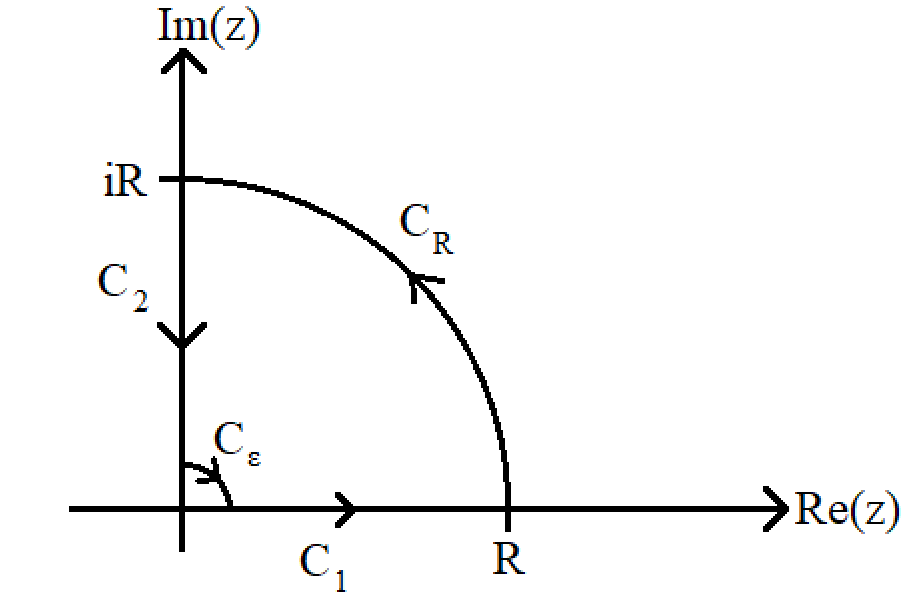
\includegraphics[scale = 0.3]{semicircle_contour.PNG}
        \end{center}

        By Cauchy's theorem, we have
        \[\oint_C f(z) = 0.\]
        On $C_{\varepsilon}$, parameterize $z = \varepsilon e^{i\theta}$, $dz = \varepsilon i e^{i\theta}d\theta$ and so
        \begin{align*}
            \int_{C_{\varepsilon}} f(z) &= \int_{\pi/2}^0\frac{e^{ik\varepsilon e^{i\theta}}}{\sqrt{\varepsilon}e^{i\theta/2}}\varepsilon i e^{i\theta}d\theta\\
            \implies \left|\int_{C_{\varepsilon}} f(z)\right| &\leq \sqrt{\varepsilon}\int_0^{\pi/2}e^{-k\varepsilon \sin(\theta)}d\theta\\
            &\leq \sqrt{\varepsilon}\int_0^{\pi/2}e^{-2k\varepsilon\theta/\pi}d\theta\\
            &= -\frac{\pi}{2k\sqrt{\varepsilon}}\left[e^{- 2k\varepsilon\theta/\pi}\right]\bigg|_0^{\pi/2}\\
            &= -\frac{\pi}{2k}\frac{e^{-k\varepsilon} - 1}{\sqrt{\varepsilon}} \to 0 \hspace{0.4cm} \text{as} \hspace{0.4cm} \varepsilon \to 0.
        \end{align*}
        On $C_R$, parameterize $z = Re^{i\theta}$, $dz = Rie^{i\theta}d\theta$ so that
        \begin{align*}
            \int_{C_R}f(z) &= \int_0^{\pi/2}\frac{e^{ikR e^{i\theta}}}{\sqrt{R}e^{i\theta/2}}Rie^{i\theta}d\theta\\
            \implies \left|\int_{C_R}f(z)\right| &\leq \sqrt{R}\int_0^{\pi/2}e^{-kR\sin(\theta)}d\theta\\
            &\leq \sqrt{R}\int_0^{\pi/2} e^{-2kR\theta/\pi}d\theta\\
            &= -\frac{\pi}{2k\sqrt{R}}\left[e^{-2kR\theta/\pi}\right]\bigg|_0^{\pi/2}\\
            &= -\frac{\pi}{2k}\frac{e^{-kR} - 1}{\sqrt{R}} \to 0 \hspace{0.4cm} \text{as} \hspace{0.4cm} R \to \infty.
        \end{align*}
        And as $R \to \infty$, $\varepsilon \to 0$, we have
        \begin{align*}
            \int_{C_1}f(z) &\to \int_0^{\infty} \frac{e^{ikx}}{\sqrt{x}}dx\\
            \int_{C_2}f(z) &\to e^{i\pi/4}\int_{\infty}^0 \frac{e^{-kx}}{\sqrt{x}}dx\\
            &= -\frac{e^{i\pi/4}}{\sqrt{k}}\int_0^{\infty}u^{-1/2}e^{-u}du\\
            &= -\frac{e^{i\pi/4}}{\sqrt{k}}\Gamma\left(\frac{1}{2}\right)\\
            &= -\sqrt{\frac{\pi}{k}}e^{i\pi/4}
        \end{align*}
        so that 
        \[\int_0^{\infty} \frac{e^{ikx}}{\sqrt{x}}dx = \sqrt{\frac{\pi}{k}}e^{i\pi/4}\]
        and since ${\displaystyle \int_0^{1}\frac{e^{-kx}}{\sqrt{x}}dx \sim \int_0^{\infty} \frac{e^{-kx}}{\sqrt{x}}dx }$ as $k \to \infty$, using our work above, we conclude 
        \[\int_0^1\frac{e^{ikx}}{\sqrt{x}}dx \sim \int_0^{\infty} \frac{e^{ikx}}{\sqrt{x}}dx = \sqrt{\frac{\pi}{k}}e^{i\pi/4} \hspace{0.4cm} \text{as} \hspace{0.4cm} k \to \infty\]
        as desired.
        
        
        \item[(c)] Deduce that
        \[\int_0^1 \sqrt{t}e^{ikt}dt \sim \frac{-ie^{ik}}{k} + \frac{\sqrt{\pi}e^{3i\pi/4}}{2k^{3/2}}\]
        as $k \to \infty$.
        \newline\newline
        \textit{Soln.} Putting parts (a) and (b) together, we have
        \begin{align*}
            \int_0^1 \sqrt{t}e^{ikt}dt &\sim -\frac{i}{k}e^{ik} + \frac{i}{2k}\sqrt{\frac{\pi}{k}}e^{i\pi/4}\\
            &= -\frac{i}{k}e^{ik} + \frac{\sqrt{\pi}}{2k^{3/2}}e^{3i\pi/4}
        \end{align*}
        as desired.
    \end{itemize}

    \pagebreak

    \item[6.3.3] Use the method of stationary phase to find the leading behavior of the following integrals as $k \to \infty$:
    \begin{itemize}
        \item[(a)] ${\displaystyle \int_0^1 \tan(t) e^{ikt^4} dt}$
        \newline\newline
        \textit{Soln.} Let $\phi(t) = t^4$. Then $\phi'(t) = 4t^3$ and so $\phi'(t) = 0 \implies t = 0$. Thus $t = 0$ is a stationary point of $\phi(t)$. We wish find an expansion for $\tan(t)$ near $t = 0$. Well,
        \begin{align*}
            \tan(t) &= \frac{\sin(t)}{\cos(t)}\\
            &= \frac{t - \tfrac{t^3}{6} + \cdots}{1 - \tfrac{t^2}{2} + \cdots}\\
            &= \left(t - \frac{t^3}{6} + \cdots\right)\left(1 + \frac{t^2}{2} + \cdots\right)\\
            &= t + \frac{t^3}{3} + \cdots
        \end{align*}
        \[\tan(t) = t + \frac{t^3}{3} + \cdots.\]
        Thus, near $t = 0$,
        \[\tan(t) \sim t\]
        and so 
        \[\int_0^1\tan(t) e^{ikt^4}dt \sim \int_0^1 te^{ikt^4}dt.\]
        To find an asymptotic expansion for the above integral, consider the function $f(z) = ze^{ikz^4}$ over the contour 

        \begin{center}
            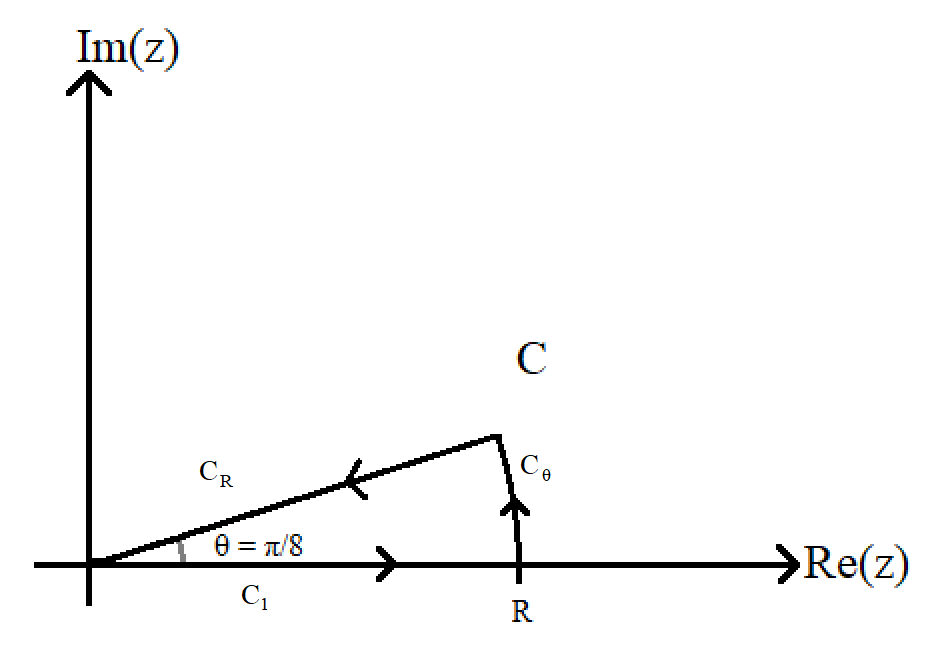
\includegraphics[scale = 0.3]{sector_contour.PNG}
        \end{center}

        By Cauchy's theorem, we have
        \[\oint_C f(z) = 0\]
        and so
        \[\int_{C_1} f(z) = \int_{-C_{\theta}} f(z) + \int_{-C_R} f(z).\]
        On $C_1$, parameterize $z = t \in \mathbb{R}$ so that 
        \[\int_{C_1}f(z) = \int_0^R te^{ikt^4}dt.\]
        On $C_{\theta}$, parameterize $z = te^{i\pi/8}$ so that 
        \[\int_{C_{\theta}}f(z) = e^{i\pi/4}\int_R^0 te^{-kt^4} dt.\]
        So that as $R \to \infty$, we have
        \begin{align*}
            \int_{C_1} &\to \int_0^{\infty}te^{ikt^4}dt\\
            \int_{C_{\theta}} &\to -e^{i\pi/4}\int_0^{\infty} te^{-kt^4}dt
        \end{align*}
        On $C_R$, parameterize $z = Re^{i\theta}$, $0 \leq \theta \leq \frac{\pi}{8}$. Then 
        \begin{align*}
            \int_{C_R} f(z) &= R^2i\int_0^{\pi/8}e^{2i\theta}e^{iR^4e^{i4\theta}}d\theta\\
            \implies \left|\int_{C_R}f(z)\right| &\leq R^2\int_0^{\pi/8}e^{-R^4\sin(4\theta)}d\theta.
        \end{align*}
        And note that $\sin(4\theta) \geq \frac{8}{\pi}\theta$ for $0 \leq \theta \leq \frac{\pi}{8}$ hence
        \begin{align*}
            R^2\int_0^{\pi/8} e^{-R\sin(4\theta)}d\theta &\leq R^2\int_0^{\pi/8} e^{-\tfrac{8R^4}{\pi}\theta}d\theta\\
            &= \frac{\pi}{8R^2}\left[e^{-\frac{8R^4}{\pi}\theta}\right]\bigg|_0^{\pi/8}\\
            &= \frac{\pi}{8R^2}\left[e^{-R^4} - 1\right]\\
            &\to 0 \hspace{0.3cm} \text{as} \hspace{0.3cm} R \to \infty.
        \end{align*}
        Thus, as $R \to \infty$, 
        \[\int_0^{\infty}te^{ikt^4}dt = e^{i\frac{\pi}{4}}\int_0^{\infty} te^{-kt^4}dt.\]
        For the right hand side integral, let $u = kt^4$, so that $du = 4kt^3dt$ and so 
        \begin{align*}
            e^{i\pi/4}\int_0^{\infty}te^{-kt^4}dt &= \frac{e^{i\pi/4}}{4k}\int_0^{\infty} \left(\frac{u}{k}\right)^{1/4}e^{-u}\left(\frac{u}{k}\right)^{-3/4}du\\
            &= \frac{e^{i\pi/4}}{4\sqrt{k}}\int_0^{\pi}u^{-1/2}e^{-u}du\\
            &= \frac{e^{i\pi/4}}{4\sqrt{k}}\Gamma\left(\frac{1}{2}\right)\\
            &= \frac{1}{4}\sqrt{\frac{\pi}{k}}e^{i\pi/4}.
        \end{align*}
        Now, by Laplace's method, we have
        \[\int_0^{1}te^{-kt^4}dt \sim \int_0^{\infty} te^{-kt^4} dt\]
        and by our work above, we have
        \begin{align*}
            \int_0^1\tan(t)e^{ikt^4}dt &\sim \frac{1}{4}\sqrt{\frac{\pi}{k}}e^{i\pi/4}.
        \end{align*}
    \end{itemize}

    \pagebreak

    \item[6.3.6] 
    \begin{itemize}
        \item[(a)] Show that the integral ${\displaystyle \int_{-\infty}^{\infty} \frac{\cos(kx)}{\cosh(x)}dx }$ has a vanishing power series, $I(k) = \mathcal{O}\left(\frac{1}{k^n}\right)$ for all $n$, as $k \to \infty$. Use contour integration to establish that $I(k) = \frac{\pi}{2}\text{sech}\left(\frac{k\pi}{2}\right) \sim \pi e^{-k\pi/2}$.
        \newline\newline
        \textit{Proof:} We begin by showing that the above integral converges. Notice
        \[\left|\int_{-\infty}^{\infty}\frac{\cos(kx)}{\cosh(x)}dx\right| \leq \int_{-\infty}^{\infty}\text{sech}(x)dx = \frac{\pi}{2}.\]
        The final equality will be shown towards the end of the problem.
        
        
        Consider the function $f(z) = \frac{e^{ikz}}{\cosh(z)}$ over the contour 

        \begin{center}
            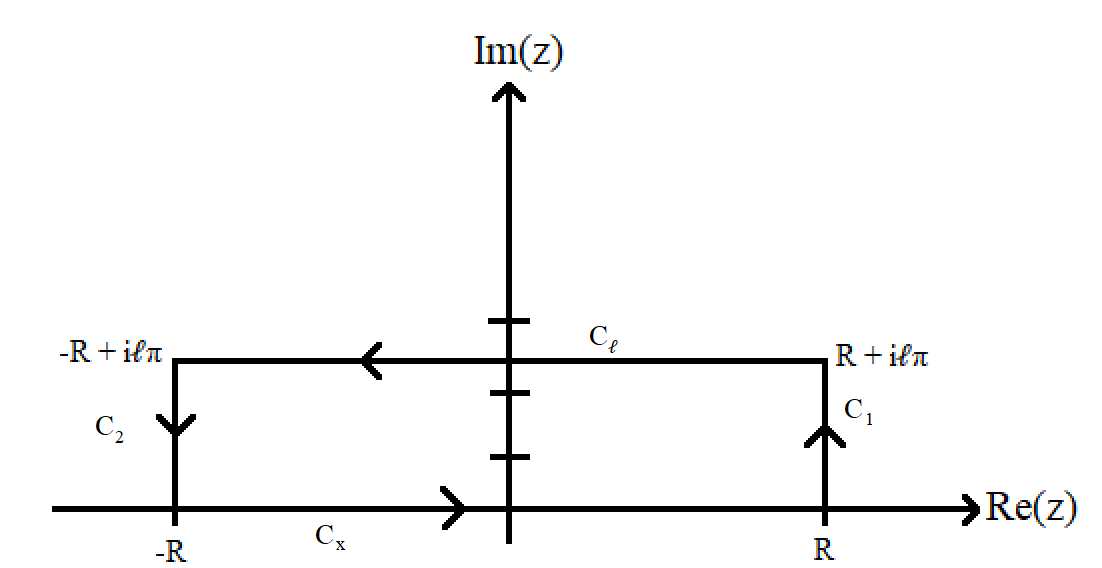
\includegraphics[scale = 0.3]{box_contour.PNG}
        \end{center}

        Note that $\cosh(z)$ has zeros on the imaginary axis since $\cosh(iy) = \cos(y) = 0$ whenever $y = \frac{\pi}{2} + \pi n$, $n \in \mathbb{Z}$, hence $\frac{1}{\cosh(z)}$ has poles on the imaginary axis. Further, these are simple poles, which we show below. The top part of the contour in the figure above is chosen such that for each $\ell \in \mathbb{N}$, the top part lies in between two poles. Note that 
        \begin{align*}
            \frac{d}{dz} \cosh(z) &= \sinh(z)\\
            \frac{d}{dz} \sinh(z) &= \cosh(z)\\
            &\vdots
        \end{align*}
        so that the Taylor expansion for $\cosh(z)$ about $z = i(\frac{\pi}{2} + n \pi)$ is given by
        \begin{align*}
            \cosh(z) &= \cosh\left(i\left(\frac{\pi}{2} + n\pi\right)\right) + \sinh\left(i\left(\frac{\pi}{2} + n\pi\right)\right)\left(z - i\left(\frac{\pi}{2} + n\pi\right)\right) + \cdots\\
            &= (-1)^ni\left[\left(z - i\left(\frac{\pi}{2} + n\pi\right)\right) - \frac{\left(z - i\left(\frac{\pi}{2} + n\pi\right)\right)^3}{3!} + \cdots\right]\\
            &= (-1)^ni\left(z - i\left(\frac{\pi}{2} + n\pi\right)\right)\left[1 - \frac{\left(z - i\left(\frac{\pi}{2} + n\pi\right)\right)^2}{3!} + \cdots\right]
        \end{align*}
        so that $\frac{1}{\cosh(z)}$ has simple poles at $z = i\left(\frac{\pi}{2} + n\pi\right)$. Now, by Cauchy's Residue Theorem, we have
        \[\oint_Cf(z) = 2\pi i \sum_{m = 0}^{\ell} \Res{i\left(\frac{\pi}{2} + m\pi\right)}f(z).\]
        And the residues are given by
        \begin{align*}
            \Res{i\left(\frac{\pi}{2} + n\pi\right)}f(z) &= \lim_{z \to i\left(\frac{\pi}{2} + n\pi\right)}\left(z - i\left(\frac{\pi}{2} + n\pi\right)\right)\frac{e^{ikz}}{\cosh(z)}\\
            &= \lim_{z \to i\left(\frac{\pi}{2} + n\pi\right)}\left(z - i\left(\frac{\pi}{2} + n\pi\right)\right)\frac{e^{ikz}}{(-1)^ni\left(z - i\left(\frac{\pi}{2} + n\pi\right)\right)\left[1 - \frac{\left(z - i\left(\frac{\pi}{2} + n\pi\right)\right)^2}{3!} + \cdots\right]}\\
            &= \frac{e^{-k\left(\frac{\pi}{2} + n\pi\right)}}{i(-1)^n\left(1 - \frac{\left(z - i\left(\frac{\pi}{2} + n \pi\right)\right)^2}{3!} + \cdots\right)}\\
            &= \frac{(-1)^n}{i}e^{-k\left(\frac{\pi}{2}+n\pi\right)}.
        \end{align*}
        Thus
        \[\oint_C f(z) = 2\pi e^{-k\frac{\pi}{2}}\sum_{m = 0}^{\ell}(-1)^me^{-k\pi m}.\]
        Taking $R, \ell \to \infty$ gives 
        \[\oint_C f(z) = 2\pi e^{-k\frac{\pi}{2}}\sum_{n = 0}^{\infty} (-1)^ne^{-k\pi n}.\]
        We now analyze the separate pieces of the contour as $R, \ell \to \infty$. On $C_1$, parameterize $z = R + iy$, $dz = idy$ so that
        \begin{align*}
            \int_{C_1}f &= i\int_0^{\ell} \frac{e^{ik(R + iy)}}{\cosh(R + iy)}dy\\
            \implies \left|\int_{C_1}f\right| &\leq \int_0^{\ell} \frac{e^{-ky}}{|\cosh(R + iy)|}dy.
        \end{align*}
        By the reverse triangle inequality, we have
        \begin{align*}
            |\cosh(R + iy)| &= \left|\frac{e^{R + iy} + e^{-R - iy}}{2}\right|\\
            &\geq \frac{1}{2}\left||e^{R + iy}| - |e^{-R - iy}|\right|\\
            &= \frac{1}{2}\left|e^{R} - e^{-R}\right|\\
            &= \frac{e^R - e^{-R}}{2}\\
            &= \sinh(R)\\
            \implies \frac{1}{|\cosh(R + iy)|} &\leq \frac{1}{\sinh(R)}.
        \end{align*}
        Thus
        \begin{align*}
            \left|\int_{C_1}f\right| &\leq \frac{1}{\sinh(R)}\int_0^{\ell}e^{-ky}dy\\
            &= \frac{-1}{k\sinh(R)}\left[e^{-ky}\right]\bigg|_0^{\ell}\\
            &= \frac{-1}{k\sinh(R)}\left[e^{-\ell y} - 1\right]\\
            &\to 0 \hspace{0.4cm} \text{as} \hspace{0.4cm} R \to \infty.
        \end{align*}
        Similarly, on $C_2$, parameterize $z = -R + iy$, $dz = idy$ so that 
        \[\int_{C_2}f(z) = i\int_{\ell}^0 \frac{e^{ik(-R + iy)}}{\cosh(-R + iy)}dy.\]
        Then
        \begin{align*}
            \left|\int_{C_2}f(z)\right| &\leq\int_0^{\ell} \frac{e^{-ky}}{|\cosh(-R + iy)|}dy.
        \end{align*}
        By the reverse triangle inequality, we find
        \begin{align*}
            |\cosh(-R + iy)| &\geq \left|\frac{e^{-R + iy} + e^{R - iy}}{2}\right|\\
            &= \frac{1}{2}\left||e^{-R + iy}| - |e^{R - iy}|\right|\\
            &= \frac{1}{2}\left|e^{R} - e^{-R}\right|\\
            &= \sinh(R)\\
            \implies \frac{1}{|\cosh(-R + iy)|} &\leq \frac{1}{\sinh(R)}
        \end{align*}
        thus, by the same argument as for $C_1$, we have
        \[\left|\int_{C_2}f(z)\right| \to 0 \hspace{0.4cm} \text{as} \hspace{0.4cm} R \to \infty.\]
        On $C_{\ell}$, parameterize $z = x + i\ell\pi$, $dz = dx$ so that
        \begin{align*}
            \int_{C_{\ell}}f(z) &= \int_{\infty}^{-\infty}\frac{e^{ik(x + i\ell)}}{\cosh(x + i\ell\pi)}dx\\
            \implies \left|\int_{C_{\ell}}f\right| &\leq e^{-k\ell}\int_{-\infty}^{\infty}\frac{1}{|\cosh(x + i\ell\pi)|}dy
        \end{align*}
        and note the following:
        \begin{align*}
            \cosh(x + i\ell\pi) &= \frac{e^{x + i\ell\pi} + e^{-x - i\ell\pi}}{2}\\
            &= \frac{e^{2i\ell\pi}e^x + e^{-x}}{2e^{-i\ell\pi}}\\
            &= e^{i\ell\pi}\frac{e^x + e^{-x}}{2}\\
            &=  (-1)^{\ell}\cosh(x)\\
            \implies |\cosh(x + i\ell\pi)| &= \cosh(x).
        \end{align*}
        Thus the integral above becomes
        \begin{align*}
            e^{-k\ell}\int_{-\infty}^{\infty}\frac{1}{|\cosh(x + i\ell \pi)|}dx &= e^{-k\ell}\int_{-\infty}^{\infty} \text{sech}(x)dx\\
            &= 2e^{-k\ell}\int_0^{\infty} \text{sech}(x)dx 
        \end{align*}
        let $u = sinh(x)$, $du = cosh(x)dx$, so that, using $\cosh^2(x) = 1 + \sinh^2(x)$, we have
        \begin{align*}
            2e^{-k\ell}\int_0^{\infty} \text{sech}(x)dx &= 2e^{-k\ell}\int_0^{\infty} \frac{1}{1 + u^2}du\\
            &= 2e^{-k\ell}\left[\tan^{-1}(u)\right]\bigg|_0^{\infty}\\
            &= \pi e^{-k\ell} \to 0 \hspace{0.4cm} \text{as} \hspace{0.4cm} \ell \to \infty.
        \end{align*}
        Thus, as $R, \ell \to \infty$,
        \[\oint_Cf(z) \to \int_{-\infty}^{\infty} \frac{e^{ikx}}{\cosh(x)}dx = \int_{-\infty}^{\infty} \frac{\cos(kx)}{\cosh(x)}dx + i\int_{-\infty}^{\infty}\frac{\sin(kx)}{\cosh(x)}dx\]
        and so
        \[\int_{-\infty}^{\infty}\frac{\cos(kx)}{\cosh(x)}dx + i\int_{-\infty}^{\infty}\frac{\sin(kx)}{\cosh(x)}dx = 2\pi e^{-k\pi/2}\sum_{n = 0}^{\infty} (-1)^ne^{-nk\pi}.\]
        Finally, we show the right hand side of the above equation equals $\pi\text{sech}\left(k\frac{\pi}{2}\right)$.
        To that end, using the exponential definition of $\text{sech}(x)$, notice for $x > 0$,
        \begin{align*}
            \text{sech}(x) &= \frac{2}{e^x + e^{-x}}\\
            &= 2e^{-x} \frac{1}{1 + e^{-2x}}\\
            &= 2e^{-x}(1 - e^{-2x} + e^{-4x} - \cdots)\\
            \implies \pi\text{sech}\left(k\frac{\pi}{2}\right) &= 2\pi e^{-k\pi/2}(1 - e^{-k\pi} + e^{-2k\pi} + \cdots)\\
            &= 2\pi e^{-k\pi/2}\sum_{n = 0}^{\infty}(-1)^ne^{-nk\pi}
        \end{align*}
        finally giving us
        \[\int_{-\infty}^{\infty}\frac{\cos(kx)}{\cosh(x)}dx = \pi\text{sech}\left(k\frac{\pi}{2}\right).\]
        Further, from our geometric expansion of $\text{sech}(x)$, we have
        \[\pi\text{sech}\left(k\frac{\pi}{2}\right) \sim \pi e^{-k\pi/2} \hspace{0.4cm} \text{as} \hspace{0.4cm} k \to \infty\]
        as desired.
    \end{itemize}
    
\end{itemize}

\end{document}
